\section{Análisis estructural}\label{sec:fea}

El diseño de este prototipo fue ampliamente debatido. Para llegar a buen puerto con las decisiones de ingeniería, lo que se utilizó fue la herramienta de elementos finitos. Más allá del buen planteo del diseño inicial, necesario para poder optimizar luego el prototipo. Un diseño malo de entrada, no hay elemento finito que lo arregle. Por esto fue crucial en base a la experiencia adquirida en estos años de estudios poder plantear un diseño inicial acorde a las necesidades en distintas circunstancias de prueba, para luego poder iterarlo. Obteniendo un coeficiente de peso y resistencia que nos sirva para poder probar el sistema de vuelo en un vehículo liviano, porque el empuje era un factor limitante, que sobreviva a los distintos escenarios y pruebas de maniobras. Para poder llegar a la finalización del proyecto en condiciones mecánicas funcionales, es decir, poder tunear de manera correcta el sistema de control sin destrozar el prototipo en el camino.

\medskip

El fuselaje fue la parte mecánica con mayor cantidad de iteraciones, se pasó por distintos prototipos. Cada uno de ellos fue pensado en el diseño intentando llevar a su geometría a la forma más eficiente pensando cómo viajaban las cargas en distintas condiciones. Para la condición de vuelo, las cargas eran el empuje del EDF y el peso  principalmente, y combinadas con los cambios bruscos de aceleración, para este caso se encontró que las limitaciones eran las geométricas. Se continuó con el modelado de la estructura imponiéndole una fuerza en la parte superior y como parámetro de decisión se utilizó el criterio que suele utilizarse en el ámbito aeroespacial que es ponerle a distintas estructuras 1 N de fuerza y ver entre ellas cuál es la más eficiente para este caso de carga. Para luego decidir entre estos prototipos y proponer una carga de prueba para comprobar que no se estaba en fluencia. Se detectó que el aterrizaje era la peor condición, así que se diseñó y modeló para este caso. Siendo el peor escenario posible caer con solo una pata a impacto y de costado, pero en el segundo rebote, es decir tocar el piso a impacto y luego al girar que soporte todo el peso del vehículo sin plastificar de costado, multiplicado por 1,4 que fue el factor de seguridad elegido (paper referencia nasa). Se decidió corroborar a fluencia la carga lateral mencionada en la pata y en el extremo superior con una carga de 100 N que resulta de multiplicar 7 Kg * 1,4 dividirlo por la gravedad y redondearlo al entero superior. En la finalización del proyecto se encontró que esta predicción fue correcta.

\medskip

Se hicieron varios modelos de distintos prototipos de fuselajes con elementos finitos, solo se muestran aquellos que nos agregaron información relevante al desarrollo de este proyecto, y las discusiones interesantes de ingeniería que en fuertes debates pudieron lograr el prototipo final .En total se han planteado 11 conjuntos de cad distintos con fuselajes distintos para luego ser modelados.

\null\newpage
\clearpage

\subsection{Modelo y simulación propuesta tipo jaula}
\begin{figure}[htb]
    \centering
    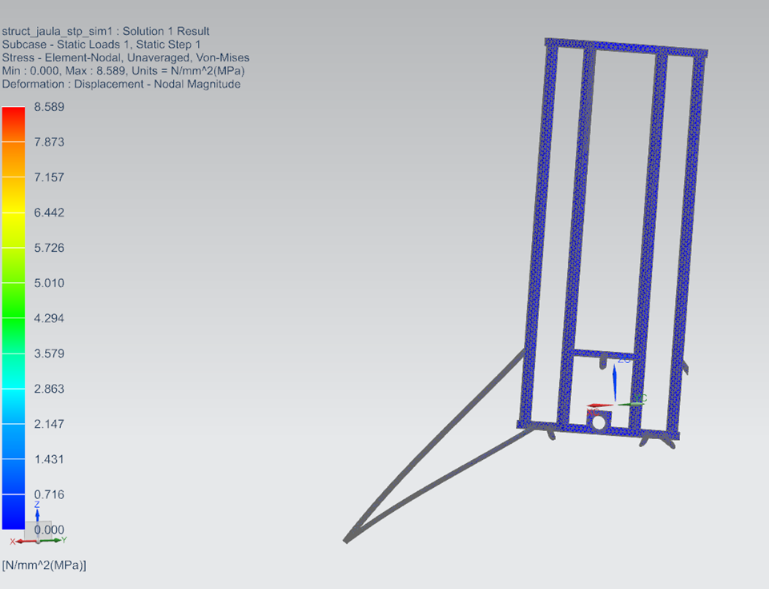
\includegraphics[width=\linewidth]{fig/fea/jaula.png}
    \caption{Modelado inicial estructura esfuerzos para carga de 1N estático en las patas dirección normal al suelo modelo de fuselaje tipo jaula.}
    \label{fig:fea/jaula}
\end{figure}

\begin{figure}[htb]
    \centering
    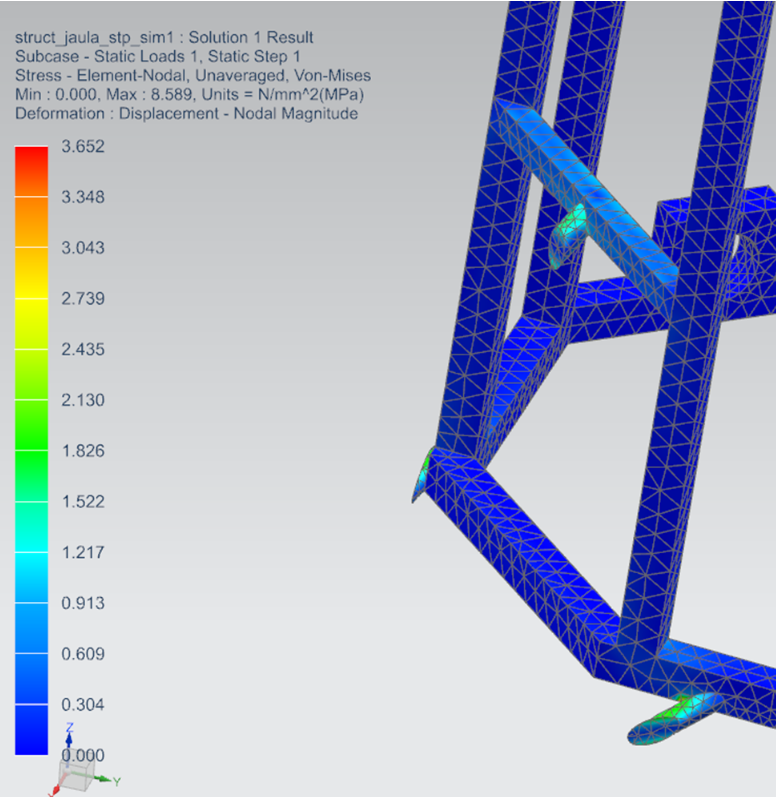
\includegraphics[width=\linewidth]{fig/fea/jaula2.png}
    \caption{Esfuerzos para carga de 1N estático para misma condición de la figura anterior pero solo vista de esfuerzos de la parte superior quitando las patas.}
    \label{fig:fea/jaula2}
\end{figure}

\null\newpage
\clearpage

\subsection{Modelo y simulación del fuselaje tubo y placas vaciadas}

\begin{figure}[htb]
    \centering
    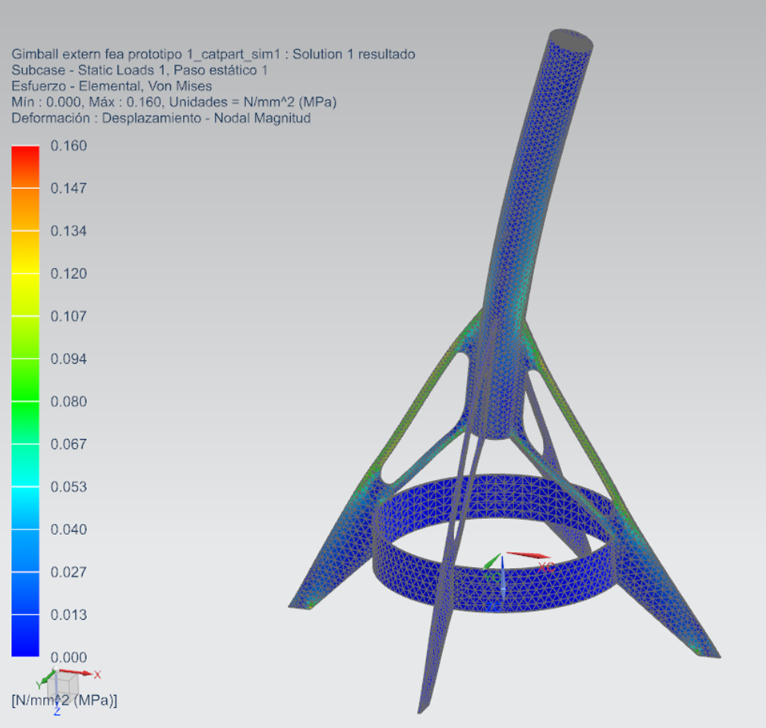
\includegraphics[width=\linewidth]{fig/fea/tuboplaca1.png}
    \caption{Modelo tubo y placas esfuerzo elemental para carga superior de 1 N en dirección planar al suelo.}
    \label{fig:fea/tuboplaca1}
\end{figure}

\begin{figure}[htb]
    \centering
    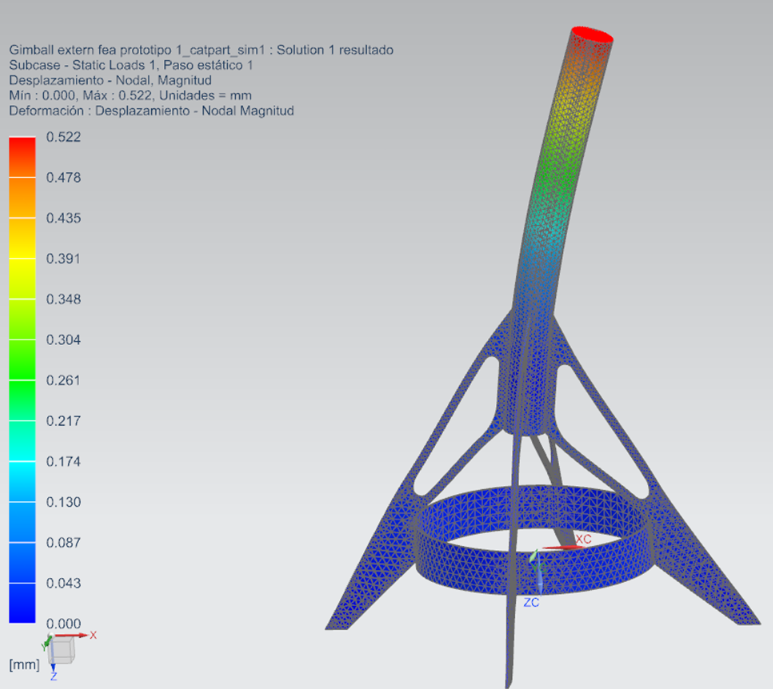
\includegraphics[width=\linewidth]{fig/fea/tuboplaca2.png}
    \caption{Modelo tubo y placas desplazamiento elemental para carga superior de 100 N en dirección planar al suelo.}
    \label{fig:fea/tuboplaca1}
\end{figure}

\begin{figure}[htb]
    \centering
    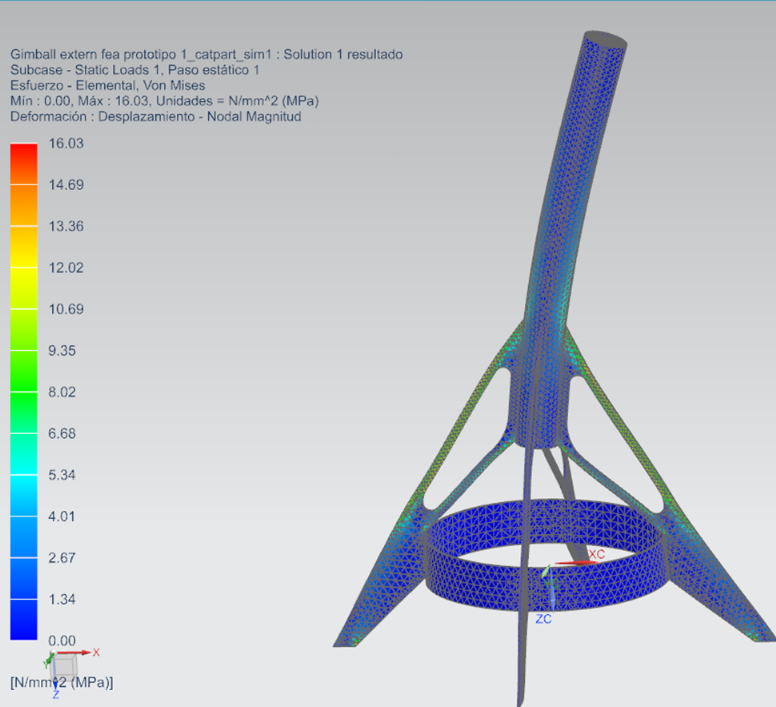
\includegraphics[width=\linewidth]{fig/fea/tuboplaca3.png}
    \caption{Modelo tubo y placas esfuerzo elemental para carga superior de 100 N en dirección planar al suelo.}
    \label{fig:fea/tuboplaca3}
\end{figure}

\begin{figure}[htb]
    \centering
    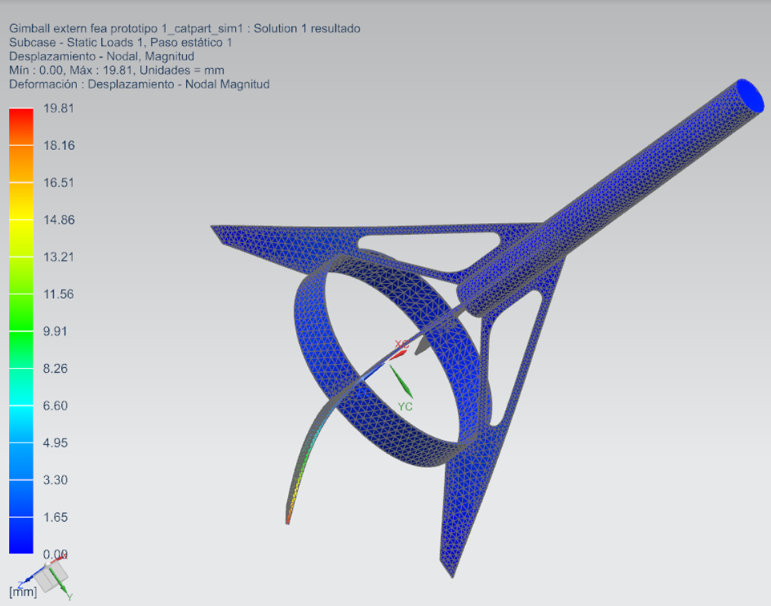
\includegraphics[width=\linewidth]{fig/fea/tuboplaca4.png}
    \caption{Modelo tubo y placas deformación en una de sus patas con una carga de 100N en dirección normal a la superficie de una de sus patas.}
    \label{fig:fea/tuboplaca4}
\end{figure}

\begin{figure}[htb]
    \centering
    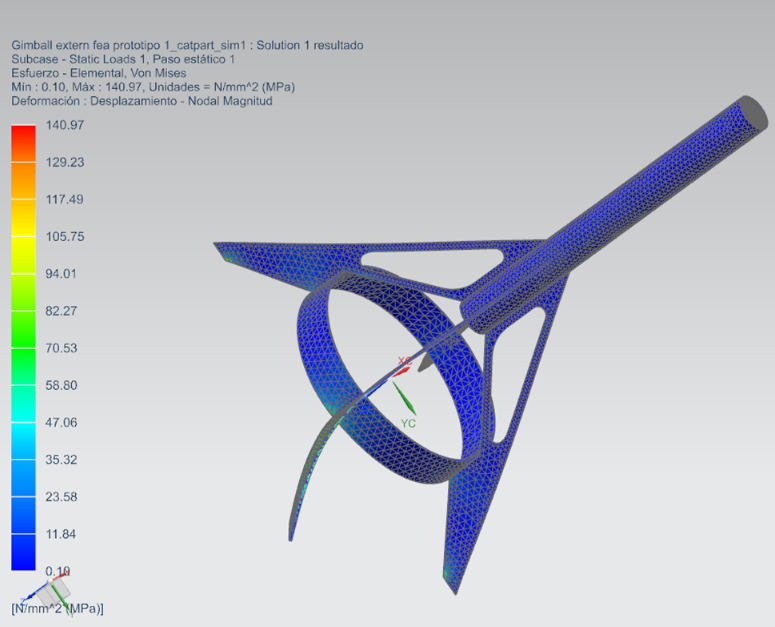
\includegraphics[width=\linewidth]{fig/fea/tuboplaca5.png}
    \caption{Modelo tubo y placas esfuerzo en una de sus patas con una carga de 100N en dirección normal a la superficie de una de sus patas.}
    \label{fig:fea/tuboplaca5}
\end{figure}

\begin{figure}[htb]
    \centering
    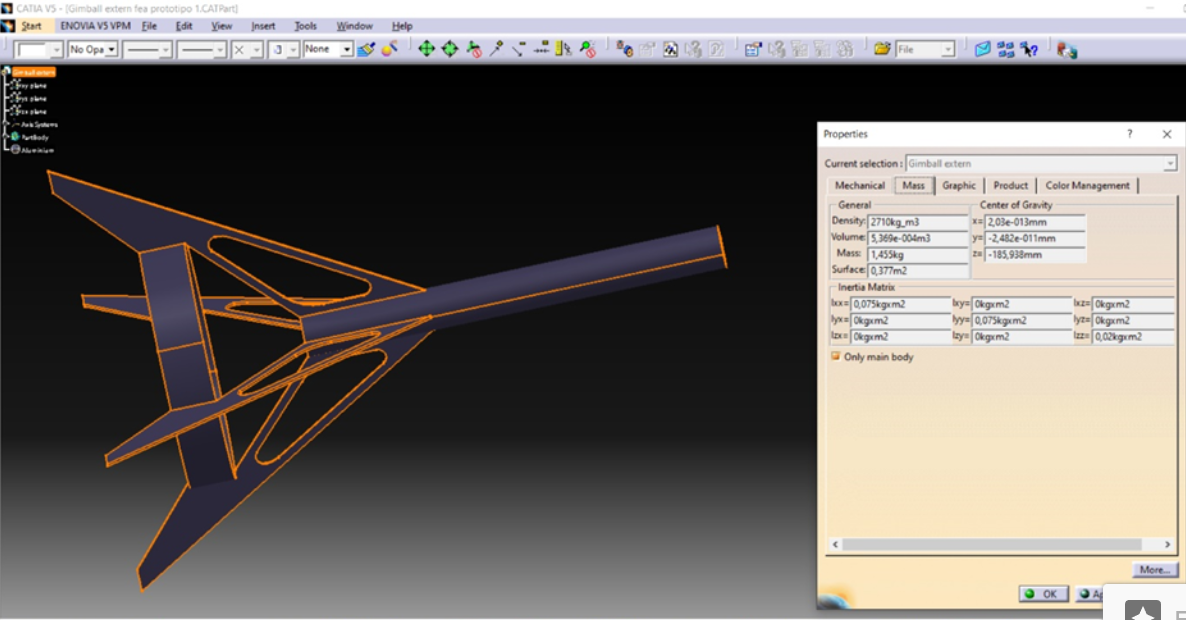
\includegraphics[width=\linewidth]{fig/fea/inercias}
    \caption{Peso e inercias del prototipo analizado.}
    \label{fig:fea/tuboplacainercias}
\end{figure}

\null\newpage
\clearpage

\subsection{Iteración del modelo y simulación en la que se definió la geometría final de las placas que componen las patas}

\begin{figure}[htb]
    \centering
    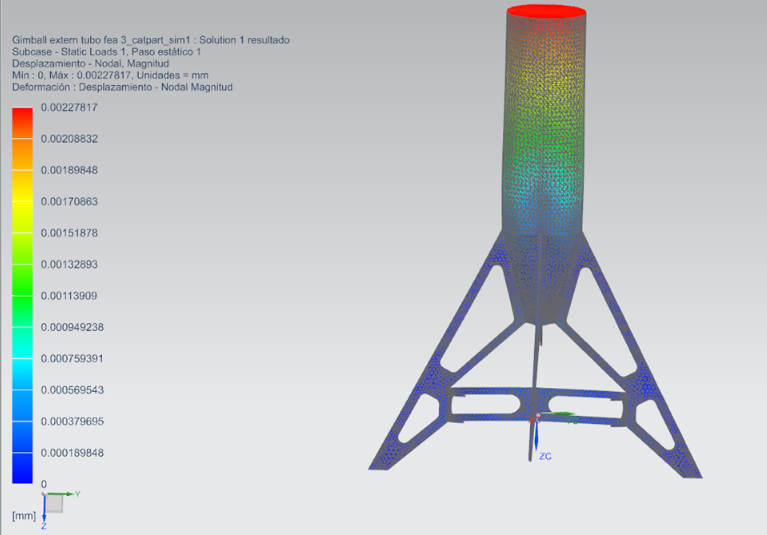
\includegraphics[width=\linewidth]{fig/fea/patas1.png}
    \caption{Modelo tubo y placas iteración $n$ desplazamiento para carga superior 1 N en dirección planar al suelo.}
    \label{fig:fea/patas1}
\end{figure}

\begin{figure}[htb]
    \centering
    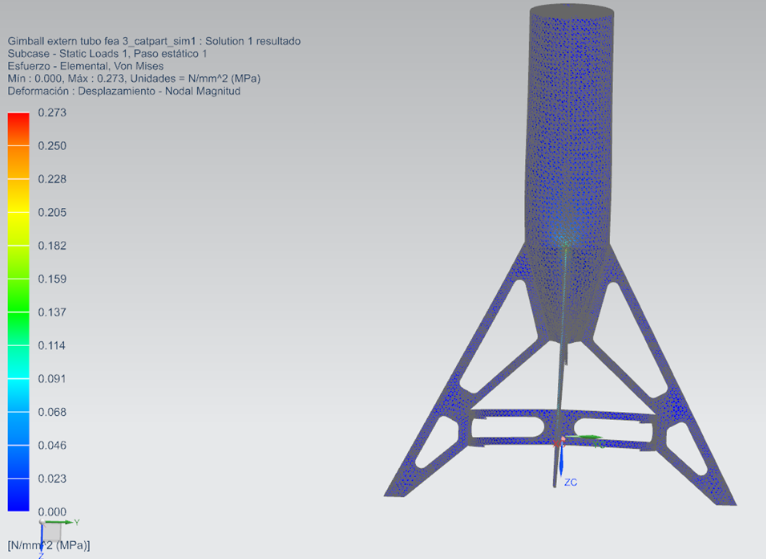
\includegraphics[width=\linewidth]{fig/fea/patas2.png}
    \caption{Modelo tubo y placas iteración $n$ esfuerzos elementales para carga superior 1 N en dirección planar al suelo.}
    \label{fig:fea/patas2}
\end{figure}

\begin{figure}[htb]
    \centering
    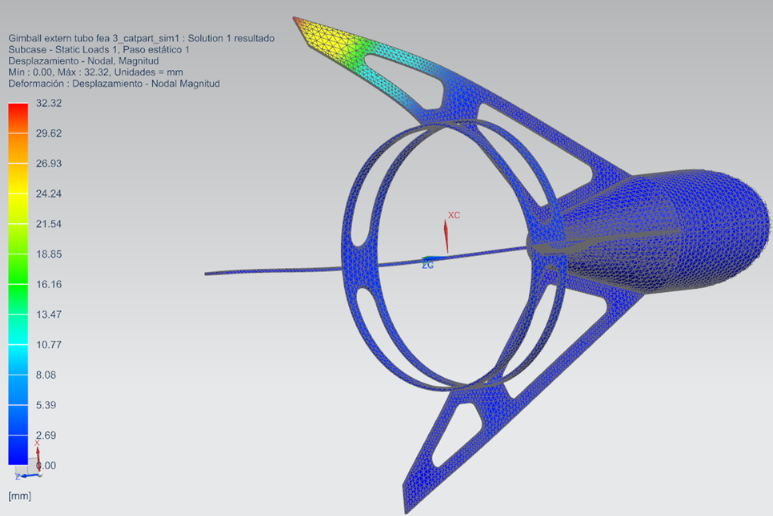
\includegraphics[width=\linewidth]{fig/fea/patas3.png}
    \caption{Modelo tubo y placas iteración $n$ desplazamientos con cargas de 100N en dirección normal a la superficie de una de sus patas.}
    \label{fig:fea/patas3}
\end{figure}


\begin{figure}[htb]
    \centering
    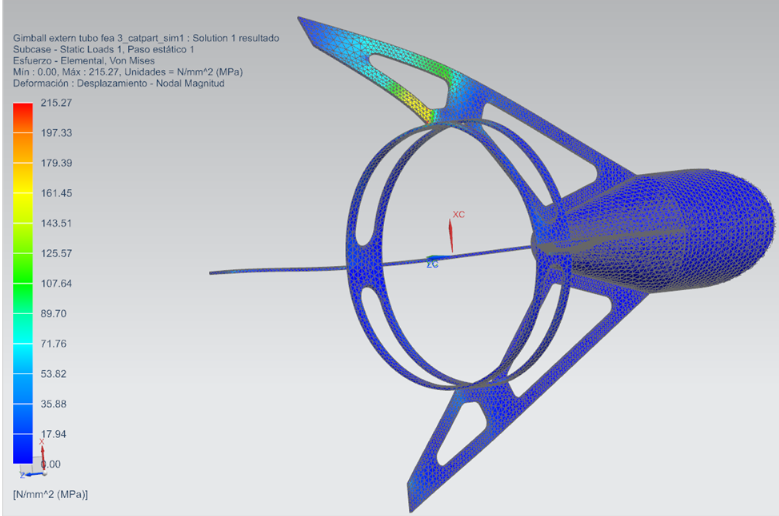
\includegraphics[width=\linewidth]{fig/fea/patas4.png}
    \caption{Modelo tubo y placas iteración $n$ esfuerzos elementales con carga de 100N en dirección normal a la superficie de una de sus patas.}
    \label{fig:fea/patas4}
\end{figure}

\begin{figure}[htb]
    \centering
    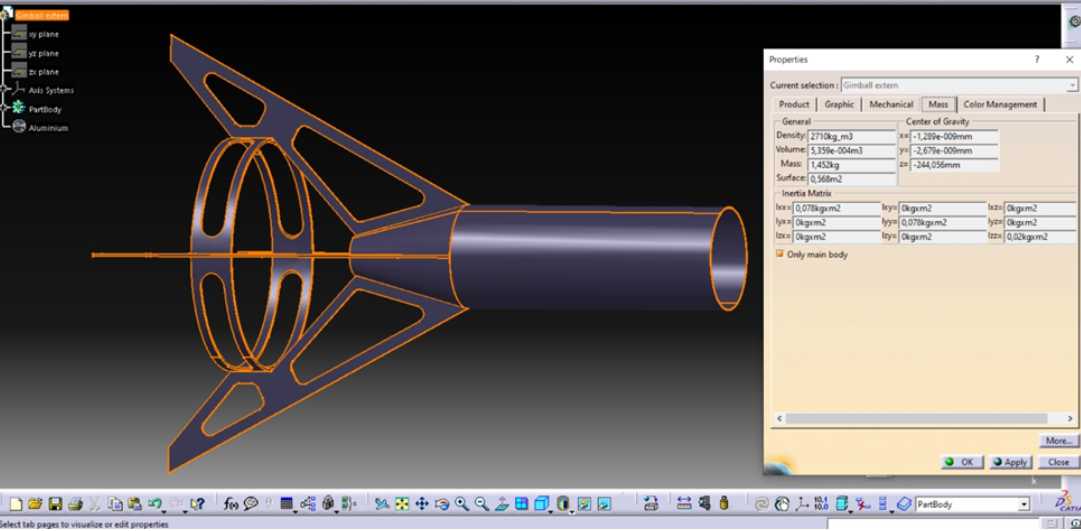
\includegraphics[width=\linewidth]{fig/fea/inerciaspatas.png}
    \caption{Peso e inercias del prototipo analizado.}
    \label{fig:fea/patas4}
\end{figure}

\begin{figure}[htb]
    \centering
    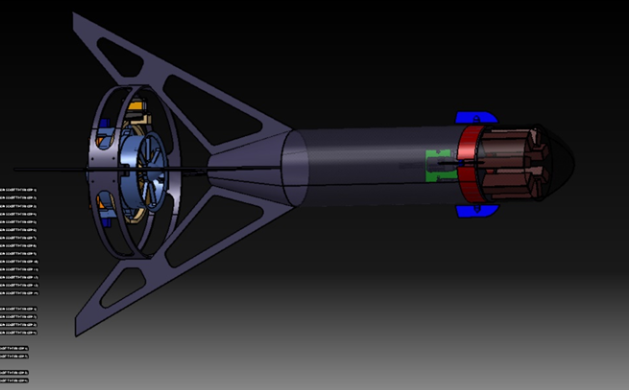
\includegraphics[width=\linewidth]{fig/fea/imagenpatas.png}
    \caption{Imagen del conjunto del prototipo del prototipo analizado.}
    \label{fig:fea/imagenpatas}
\end{figure}

\null\newpage
\clearpage

Se comprobó que las patas aguantaron las cargas de diseño para su peor condición con factor de seguridad mayor a 1.4.

Como se vio que la estructura tubular estaba sobredimensionada para ser portadora de los componentes electrónicos, sin más análisis se procedió al vaciado para poder acceder a la electrónica. Se optó por una cuestión de simplicidad y avance con los tiempos de manufactura de prescindir del cono invertido superior, quedando tubular el diseño final del fuselaje. 

